% Freshness / query latency spread, one log axis (p50, live 8-node run).
% Data: scripts/eval/out/summary.csv (E2a live, E2c live rows).
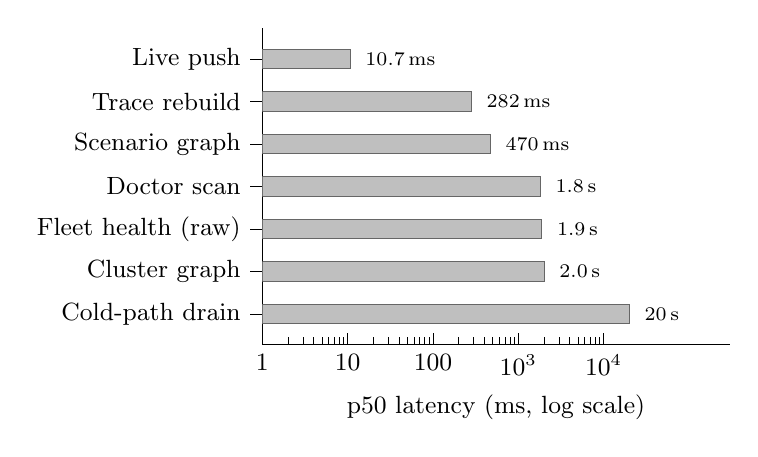
\begin{tikzpicture}
\begin{axis}[
    xbar,
    xmode=log,
    log origin=infty,
    width=0.62\linewidth,
    height=5.6cm,
    xmin=1, xmax=300000,
    xtick={1,10,100,1000,10000},
    xticklabels={1,10,100,$10^3$,$10^4$},
    xlabel={p50 latency (ms, log scale)},
    symbolic y coords={
      {Cold-path drain},
      {Cluster graph},
      {Fleet health (raw)},
      {Doctor scan},
      {Scenario graph},
      {Trace rebuild},
      {Live push}},
    ytick=data,
    y dir=normal,
    yticklabel style={font=\small},
    xticklabel style={font=\small},
    xlabel style={font=\small},
    nodes near coords,
    nodes near coords style={
      font=\scriptsize, anchor=west, xshift=2pt},
    point meta=explicit symbolic,
    bar width=7pt,
    enlarge y limits=0.12,
    axis lines*=left,
    tick style={black},
]
\addplot[fill=black!25, draw=black!60] coordinates {
  (10.7,{Live push}) [10.7\,ms]
  (282,{Trace rebuild}) [282\,ms]
  (470,{Scenario graph}) [470\,ms]
  (1807,{Doctor scan}) [1.8\,s]
  (1881,{Fleet health (raw)}) [1.9\,s]
  (2009,{Cluster graph}) [2.0\,s]
  (20000,{Cold-path drain}) [20\,s]
};
\end{axis}
\end{tikzpicture}
